\chapter{Solution development}

\section{Behaviour design}

The behavior of each robot is modeled using a non-deterministic finite state automata (\textit{NFA})(see figure \ref{fig:NFA}). Such an architecture has been chosen for the robot since its behavior is not trivial and more tasks must be executed at different times. By using a FSA, it is easy to explicitly express activities, conditions and non-deterministic transitions. Moreover, each state can be developed as a separated module, and the most suitable solution can be implemented case by case.

\noindent
The robot starts in the ``resting'' state. A non-deterministic transition makes the robot leave the base and start the exploration with a probability $P1$. 

\noindent
When exploring, the robot looks for any close landmark and, if it is the case, it joins the cluster around such landmark with a probability $P2$ and enters in ``waiting for cluster to complete" state. Moreover, the robot may quit the exploration task at any moment and return to the base with a probability $P3$. In the latter casuistry, the robot enters in the ``returning to base" state.

\noindent
When a cluster is completed by reaching the required number of robots $N$, the robot enters in the ``reconnaissance'' state. Such a state conceptually correspond to the phase during which the robots in the cluster should explore the area near the landmark. Such a task is not executed in this project for simplicity, but few different algorithms have been created to let a set of robots to explore and map a given area.

\noindent
The robot ends the reconnaissance task after $t_1$ seconds, and it returns to the base.

\noindent
When returning to the base, the robot executes a phototaxis task. The robot enters in the ``resting'' state once it is detected that it successfully returned to the base. 

\noindent
In the end, the robot may leave the cluster before it is completed with a probability $P4$. In this case, it enters in the ``biased exploration" state, that is a state where the robot executes the regular exploration tasks
but with inhibited stimuli from landmarks. After $t_2$ seconds it returns in the normal exploration behaviour. Such a intermediate state is required so that the robot may step away from the landmark (otherwise, even though it is a probabilistic transition, it would join the cluster again in most of the cases). TODO: required?  

\begin{figure}[H]
\centering
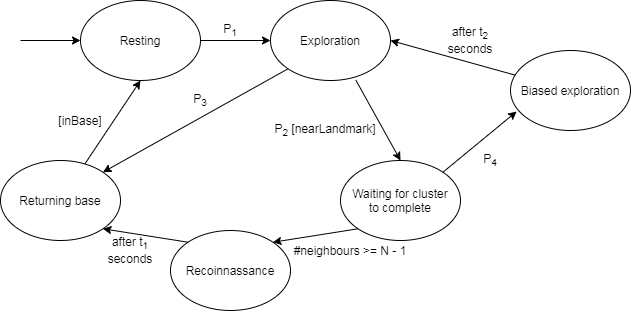
\includegraphics[width=\linewidth]{images/NFA.png}
\caption{\textit{NFA representing the behaviour of the robot. $P_i$ represent a non-deterministic transition that happens with such probability.}}
\label{fig:NFA}
\end{figure}

The implementation of the FSA is executed by using a ``states`` table to store the code be executed in each state. The variable ``current\_state'' represents the current active state, while transition are executed by checking simple``if-then-else'' conditions.

\noindent
In the end, a variable ``t'' stores the time spent by the robot in the current state.

\subsection{Motor schema design}

When a state requires motion, its design has been developed using a motor schema approach and, once the total force suffered by the robot has been calculated, the following formula is used to switch from the translational-angular model to differential one (i.e., find the velocity of each wheel out from the direction and length of the total suffered force):    

\begin{equation}
\begin{bmatrix} 
v_l \\
v_r
\end{bmatrix}
=
\begin{bmatrix} 
1 & -L/2 \\
1 & L/2
\end{bmatrix}
\begin{bmatrix} 
v \\
\omega
\end{bmatrix}
\tag{3.0}\label{eq:3.0}
\end{equation}

\noindent
where:

\smallskip
\noindent
$v_l$ = velocity of the left wheel

\noindent
$v_r$ = velocity of the right wheel

\noindent
$L$ = distance between the two wheels

\noindent
$v$ = translational velocity

\noindent
$\omega$ = angular velocity

\section{Resting}

The robot just checks if a transition to the exploration state should occur, and so no particular architectural style has been adopted for this module. The following function has been used to model the probability:

\begin{equation}
    p = tanh((t - Shift) / Patience) + 1 \tag{3.1}\label{eq:3.1}
\end{equation}

\noindent
The idea is to create a probability that is directly proportional to the time spent in the current state using a non linear relation. Moreover, the probability should grow very slowly at the beginning so that the robot will remain in the resting state for a while. 

\noindent
The function $tanh(x)$ is the basic function used to represent such relation\footnote{A reasonable alternative would be the exponential function, but it requires the tuning of few parameters so that the ``tail'' of the function take reasonable values} (figure \ref{fig:tanh}\footnote{The figure illustrates the regular \textit{tanh} function instead of the one exposed in formula \ref{eq:3.1} since the latter one, despite having a ``similar shape'', can hardly be graphically shown.}). The $Shift$ value is constant (500) so we can take the slice of the function having up concavity while dealing with positive time values. The $Patience$ value is a parameter used to tone all values down. In the end, the $+1$ factor let the function have positive values.  

\noindent
Table \ref{tab:f-values} reports few reference values of the function.

\begin{table}[H]
\centering
\begin{tabular}{| c | c |}

\hline
t & p \\
\hline
 0  & 0.013 \\
 10 & 0.015 \\
 50 & 0.022 \\
100 & 0.036 \\
500 & 1 \\
\hline

\end{tabular}
\caption{\label{tab:f-values}\textit{Few example values of the function used to model dependency with elapsed time using a non linear relation.}}
\end{table}

\begin{figure}[H]
\centering
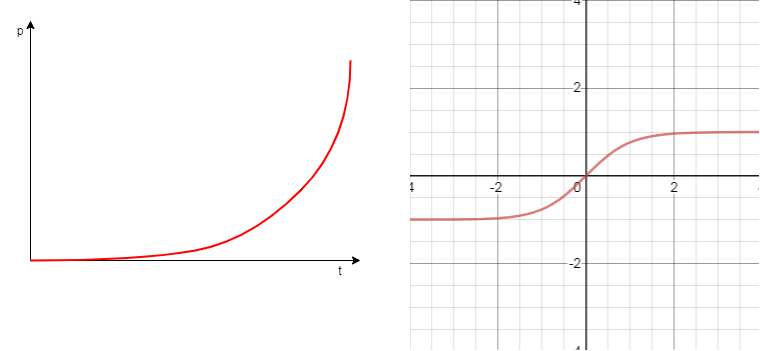
\includegraphics[width=8cm, keepaspectratio]{images/tanh.png}
\caption{\textit{Graph of the tanh function in range [-4;4].}}
\label{fig:tanh}
\end{figure}

\section{Exploration}

The robot executes a ballistic motion. A single potential field is created since the obstacle avoidance feature is implicitly given from the random walk itself. The direction of such potential field is randomly chosen each time an obstacle is detected, while its strength is given by a constant value ``CRUISE\_VELOCITY''. 

\smallskip
When exploring, the robot has a fixed probability to quit such task. Such parameter has been tuned with a very low vale (0.001) in order to avoid too much segmented behaviours where the robots keep on fluctuating just between the two states of ``exploration'' and ``returning to base''.  

\section{Clustering}

A robot may join/create a cluster when close to a landmark with a probability described by the following function:

\begin{equation}
    p =  \frac{(tanh((t - Shift) / Patience) + 1) * tanh(n / NeighborInfluenceLimiter)}{(NeighborInfluenceLimiter * PatienceEnhancer)} \tag{3.2}\label{eq:3.2}
\end{equation}

The probability is proportional to number of robots already in the cluster ($n$) and to the time spent exploring ($t$) both. The same formula in \ref{eq:3.1} has been used the time dependence term. 
The parameter $NeighborInfluenceLimiter$, as the name hints, limits the influence of number of neighbors in the final result.

\noindent
The denominator is a normalization term so reasonable values can be obtained, and it can be tuned by the parameter $PatienceEnhancer$ that makes the robot wait longer as it is increased.

\noindent
Figure \ref{fig:cluster-join} reports the graph of the function in formula \ref{eq:3.2}.

\begin{figure}[H]
\centering
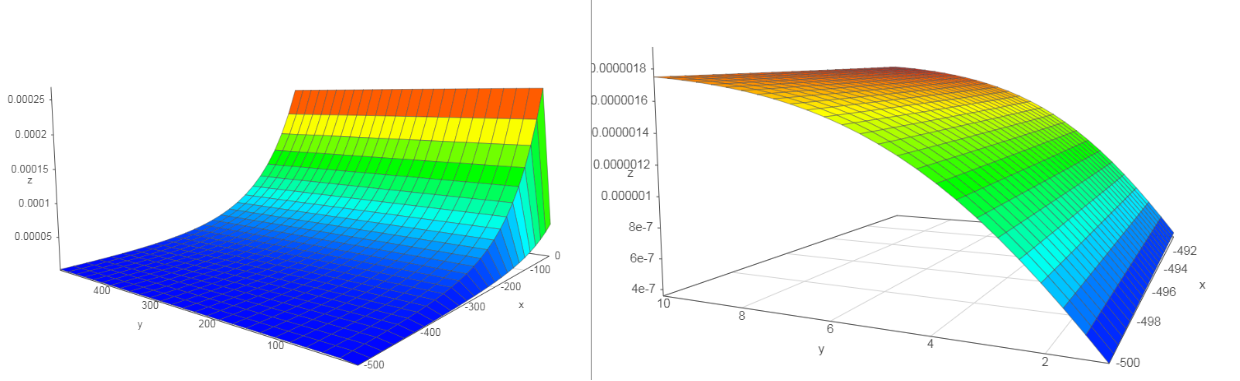
\includegraphics[width=\linewidth]{images/cluster_join.png}
\caption{\textit{x-axis = time, y-axis = number of neighbors, z-axis = probability. Graph of the plot in domain [-500;0], [1;500]  showing the total trend of the function (left) so the time relation can be shown well. On the right, a zoom in in range [-500; -492], [1:10] is executed to show the dependence upon neighbors (indeed, the number of robots in the cluster will never be about the previous order of magnitude ($10^2$) , and so low values, that cannot be appreciated in the left graph, are the the ones of interest.}}
\label{fig:cluster-join}
\end{figure}

Similarly, the probability for a robot to leave a cluster before it is completed is modeled using the following function:

\begin{equation}
    p =  \frac{(tanh((t - Shift) / Patience) + 1) / tanh(n / NeighborInfluenceLimiter)}{(NeighborInfluenceLimiter * PatienceEnhancer)} \tag{3.3}\label{eq:3.3}
\end{equation}

Formula \ref{eq:3.2} and \ref{eq:3.3} are exactly the same function except for a sign (division instead of multiplication of the two terms that model relation with time and number of neighbors). Indeed, the robot increases its probability to leave as time passes (direct proportionality) but, at the same time, its probability to leave is decreased as the number of perceived neighbors increases (inverse proportionality)(the more robots, the more probability to complete the cluster soon is the underlying reason that may lay under such behavior). 

\noindent
Figure \ref{fig:cluster-leave} reports the graph of the function in \ref{eq:3.3}.

\begin{figure}[H]
\centering
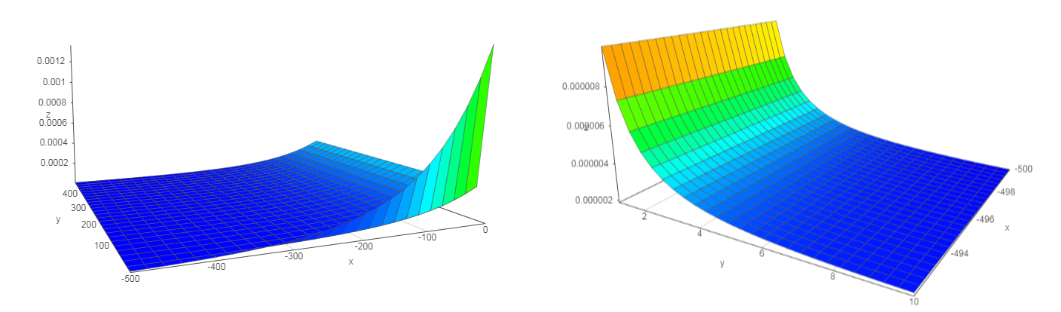
\includegraphics[width=\linewidth]{images/cluster_leave.png}
\caption{\textit{Similal reasonings of figure \ref{fig:cluster-join}. The probability slowly increases as time passes (x-axis) and rapridly decreases as numbe of neighbors increases (y-axis).}}
\label{fig:cluster-leave}
\end{figure}

\section{Returning to base}

This state must mixes phototaxis and obstacle avoidance, and so a motor schema approach has been used to easily blend such two tasks.

\smallskip
The phototaxis capability is created by using an attractive potential field produced by the light source. Hence, the resulting force, whose direction guides to robot toward the light source, has a value inversely proportional to the perceived light.

\smallskip
The obstacle avoidance capability is created by using a tangential field around any obstacle so the robot can circumnavigate boxes or other robots. By exploiting proximity sensors, a perpendicular force is created($\pi/2$ from the sensor orientation, and proportional to the proximity). A possible issue is given from the boundary walls that may create local minima in some rare cases. However, such problem may be fixed by introducing a third potential field: a perpendicular one coming from the walls. Moreover, when travelling to base, the robot should not slip into any wall in most of the cases, and so the issue is not of primary importance for the time being.
 


